%%
%% Author: Dario Chinelli
%% begin 2019-12-04
%% last mod 2022-02-02
%%

% Preamble
\documentclass[class=article, crop=false]{standalone}

% Packages
\usepackage{tikz}
\usetikzlibrary{positioning}

% Document
\begin{document}

\begin{figure}[h!]
\centering
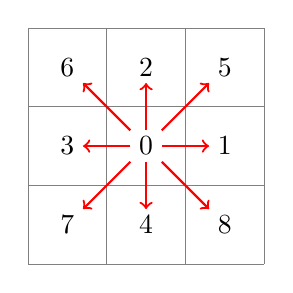
\begin{tikzpicture}
% Lines
\draw[step=1cm,gray,very thin] (0,0) grid (3,3);
\draw[thick,->,red] (1.7,1.5) -- (2.3,1.5);
\draw[thick,->,red] (1.5,1.7) -- (1.5,2.3);
\draw[thick,->,red] (1.3,1.5) -- (0.7,1.5);
\draw[thick,->,red] (1.5,1.3) -- (1.5,0.7);
\draw[thick,->,red] (1.7,1.7) -- (2.3,2.3);
\draw[thick,->,red] (1.3,1.7) -- (0.7,2.3);
\draw[thick,->,red] (1.3,1.3) -- (0.7,0.7);
\draw[thick,->,red] (1.7,1.3) -- (2.3,0.7);

% Nodes
\draw (1.5,1.5) node[black] {0};
\draw (2.5,1.5) node[black] {1};
\draw (1.5,2.5) node[black] {2};
\draw (0.5,1.5) node[black] {3};
\draw (1.5,0.5) node[black] {4};
\draw (2.5,2.5) node[black] {5};
\draw (0.5,2.5) node[black] {6};
\draw (0.5,0.5) node[black] {7};
\draw (2.5,0.5) node[black] {8};

\end{tikzpicture}
\captionsetup{width=.5\linewidth}
\caption{The possible transitions, represented as vectors. For the D2Q9 model those vector are also representing the velocity vectors.}
\label{fig:D2Q9_k_arrow}
\end{figure}

\end{document}
